\chapter{Arquitectura e implementación da aplicación}
\label{chap:implementacion_aplicacion}
Detalles da implementación do software, problemas xurdidos e solucions aplicadas
posibles subseccion:
servidor python- control das luces, control da camara, comunicacion, sockets e broadcasting
aplicacion Android- layouts e botons, comunicacions ordes e recepcion de vídeo, xestion de varios dispositivos


Son moitas as posibilidades de implementación deste dispositivo, os requisitos principais son:
\begin{itemize}
    \item Dispoñer dunha pantalla para visualizar o vídeo e o estado das luces.
    \item Contar con algunha interface de entrada de datos como botóns ou pantalla táctil.
    \item Dispoñer dun hardware para comunicarse co dispositivo principal. Como por exemplo: Wi-Fi, Bluetooth ou USB.
    \item Contar cunha batería ou fonte de alimentación
\end{itemize}

Realizar unha implementación física do dispositivo contaría coas vantaxes de poder contar cunha alta personalización dos seus compoñentes e robustez ao contar cun único dispositivo obxectivo. Sen embargo se nos presenta outra opción moito máis atractiva: utilizar un telefono móbil e crear unha aplicación dende onde poder visualizar o vídeo e controlar as luces, aparte de aforrar a construción do dispositivo. Reducirase así o número de compoñentes que o usuario ten que levar, xa que é habitual dispoñer dun móbil en todo momento.

Desenvolverase a aplicación para o sistema operativo Android xa que este é o sistema operativo máis empregado globalmente e nos permitirá chegar a un maior numero de usuarios.

Para suxeitar un teléfono móbil ao guiador da bicicleta existen múltiples ancoraxes que se adaptan a varios tamaños de teléfono. Tamén existen modelos configurables segundo o tamaño do teléfono que despois se poden imprimir en 3D.

\section{Esquema xeral da aplicación}
Para crear esta aplicación Android optarase por utilizar a linguaxe de programación Kotlin e o entorno de programación Android Studio. Kotlin é unha linguaxe de programación creada por JetBrains executable na maquina virtual de Java, dende 2017 Kotlin é unha linguaxe oficial para desenvolver aplicacións Android.

Algunhas das súas vantaxes fronte a Java son:
\begin{itemize}
    \item Unha maior expresividade: Podes escribir mais con menos código.
    \item Maior seguridade: En Kotlin e obrigatorio especificar a nulabilidade dos obxectos e esta se comproba en tempo de compilación.
    \item É funcional: Kotlin é unha linguaxe orientada a obxectos pero inclúe conceptos da programación funcional como as expresións lambda.
    \item Fai uso de extensión de funcións: Permite estender clases con novas funcionalidades se necesidade de ter aceso o código da clase.
    \item É altamente interoperable: Pódese utilizar librerías e clases de Java no mesmo proxecto.
\end{itemize}
incluír referencia a libro Kotlin

A aplicación contará con catro compoñentes. O principal será a \emph{MainActivity}, a encargada de iniciar as compoñentes a visualizar na pantalla, executar as ordes e mostrar a información. O segundo será o \emph{layout} onde se definiran as compoñentes a visualizar e a sua posición en pantalla. O terceiro a clase \emph{request} a encargada da conexión co servidor e de transmitirlle as ordes. O cuarto elemento é a clase encargada de recibir o vídeo e descodificalo.

\section{Actividade principal}
A actividade principal ou \emph{MainActivity} dunha aplicación Android é a primeira pantalla que aparece cando executase a aplicación e a encargada de controlar o seu funcionamento e a sua interface de usuario. Neste caso a actividade será a encargada de mostrar os botóns e encargarse do seu funcionamento, amosar o estado da conexión, encargarse da xestión do sensores e reproducir o vídeo. O mesmo tempo encargarase de instanciar e comunicarse coas clases encargadas da conexión co dispositivo e da recepción de vídeo.

\subsection{Layout}
Un \emph{layout} é a definición da estrutura da interface de usuario. Esta actividade contará con dous \emph{layouts} un para a posición vertical e outro para a posición horizontal da pantalla
\subsubsection{Layout vertical}
Este \emph{layout}, figura 4.1, contará cunha superficie reservada para o vídeo na metade superior da pantalla. Na metade inferior situaranse os botóns encargados de executar as ordes. Na parte superior situase a barra de estado que na sua parte dereita contará cun botón para conectar que servirá o tempo de indicador de conexión, a súa esquerda mostrarase unha barra para controlar a intensidade dos leds.
\begin{figure}[tb]
  \centering
  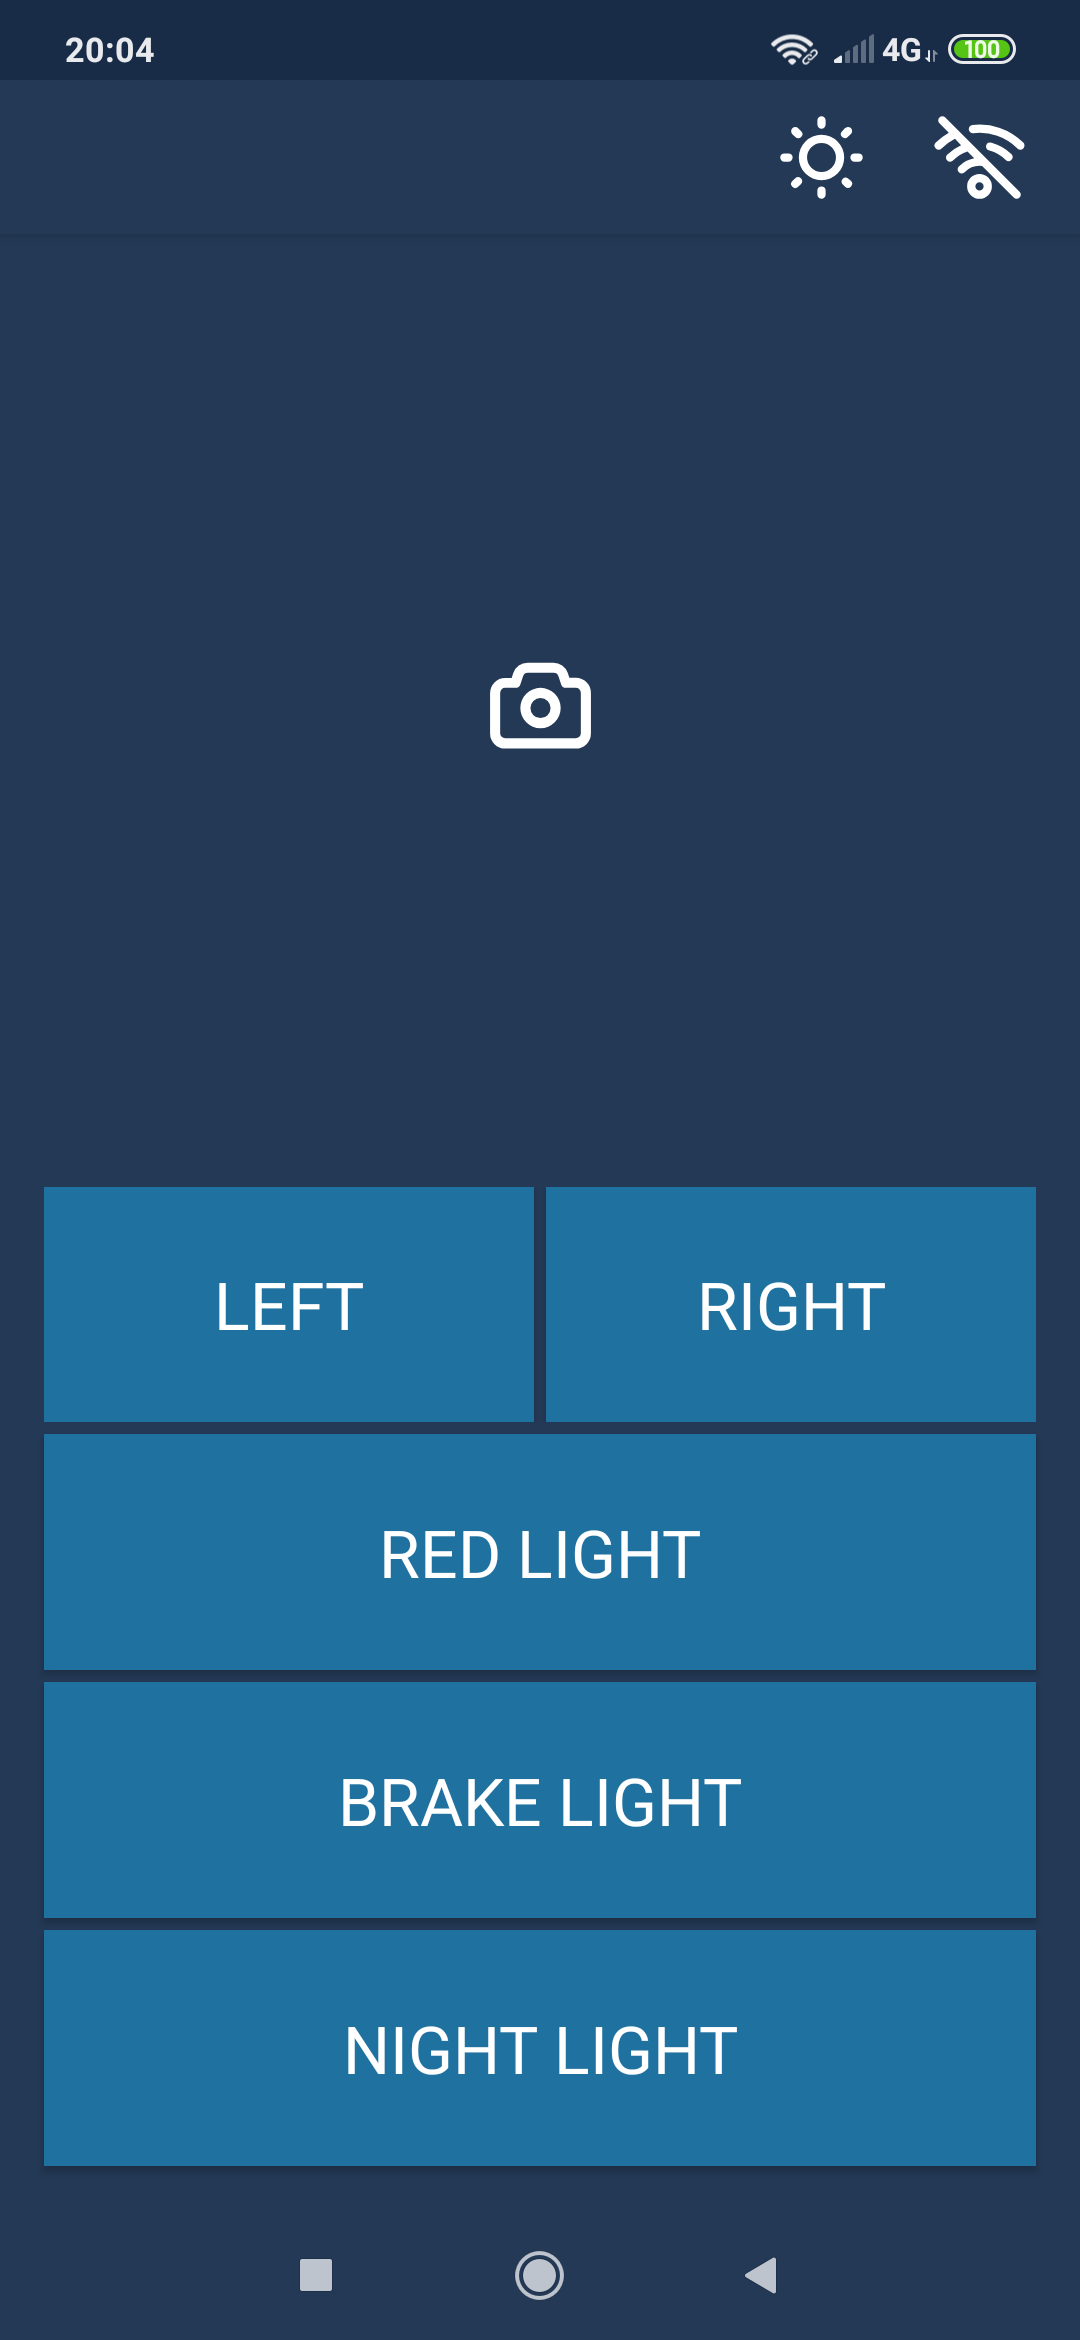
\includegraphics[scale=.1]{imaxes/layout-vertical1.png}
  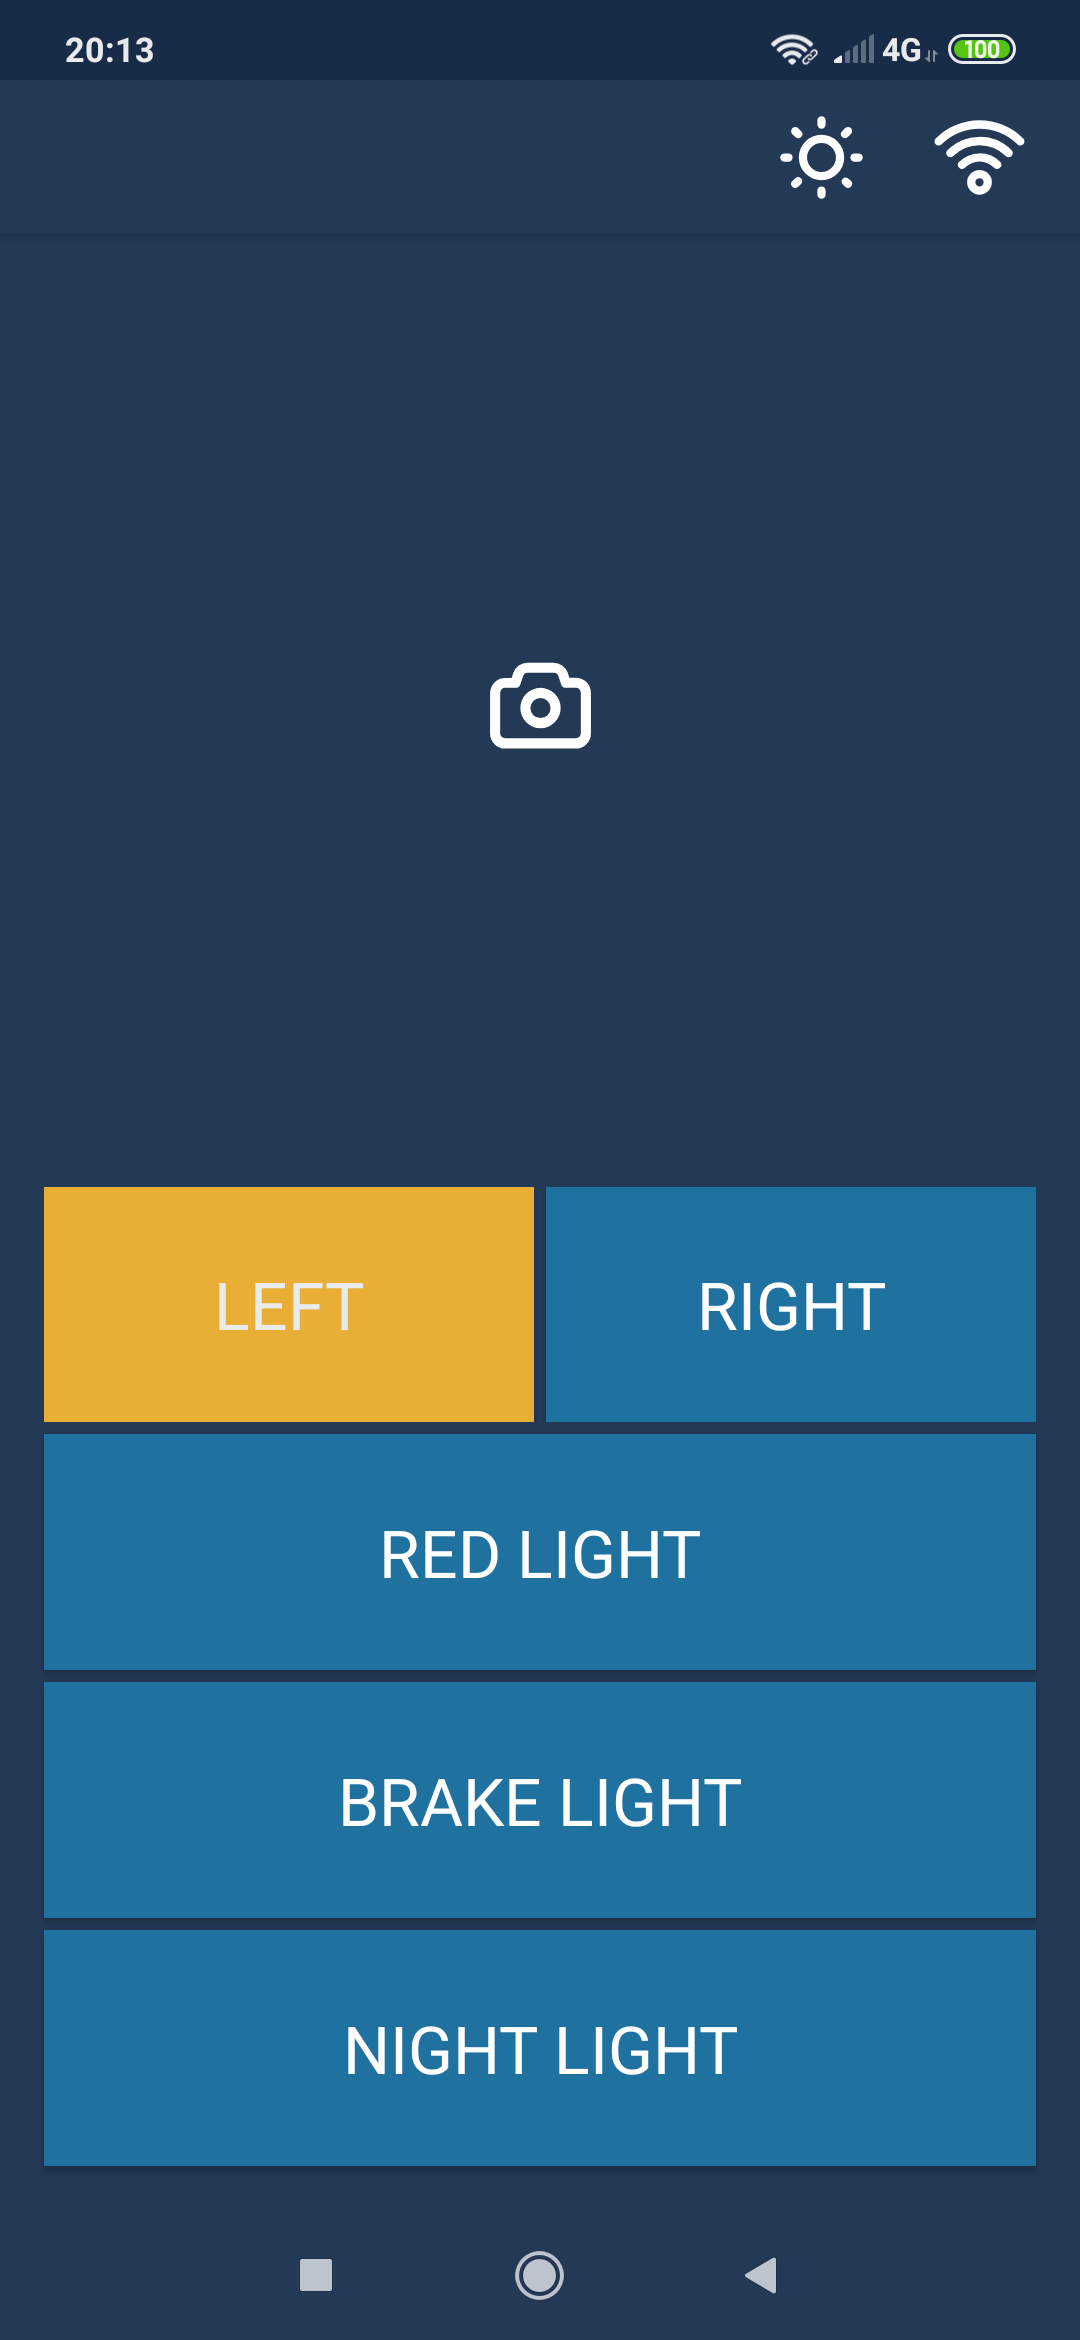
\includegraphics[scale=.1]{imaxes/layout-vertical2.png}
  \caption{Capturas de pantalla do \emph{layout} horizontal.}
  \label{f:layout horizontal}
\end{figure}
\subsubsection{Layout horizontal}
Neste \emph{layout}, figura 4.2, o vídeo mostrarase como o fondo e os botóns sobre el. Os de xiro a esquerda e xiro dereita situados a ámbolos dous lados e o resto incluíndo o de control de intensidade lumínica e o de conexión situaranse na parte de inferior da pantalla.
\begin{figure}[tb]
  \centering
  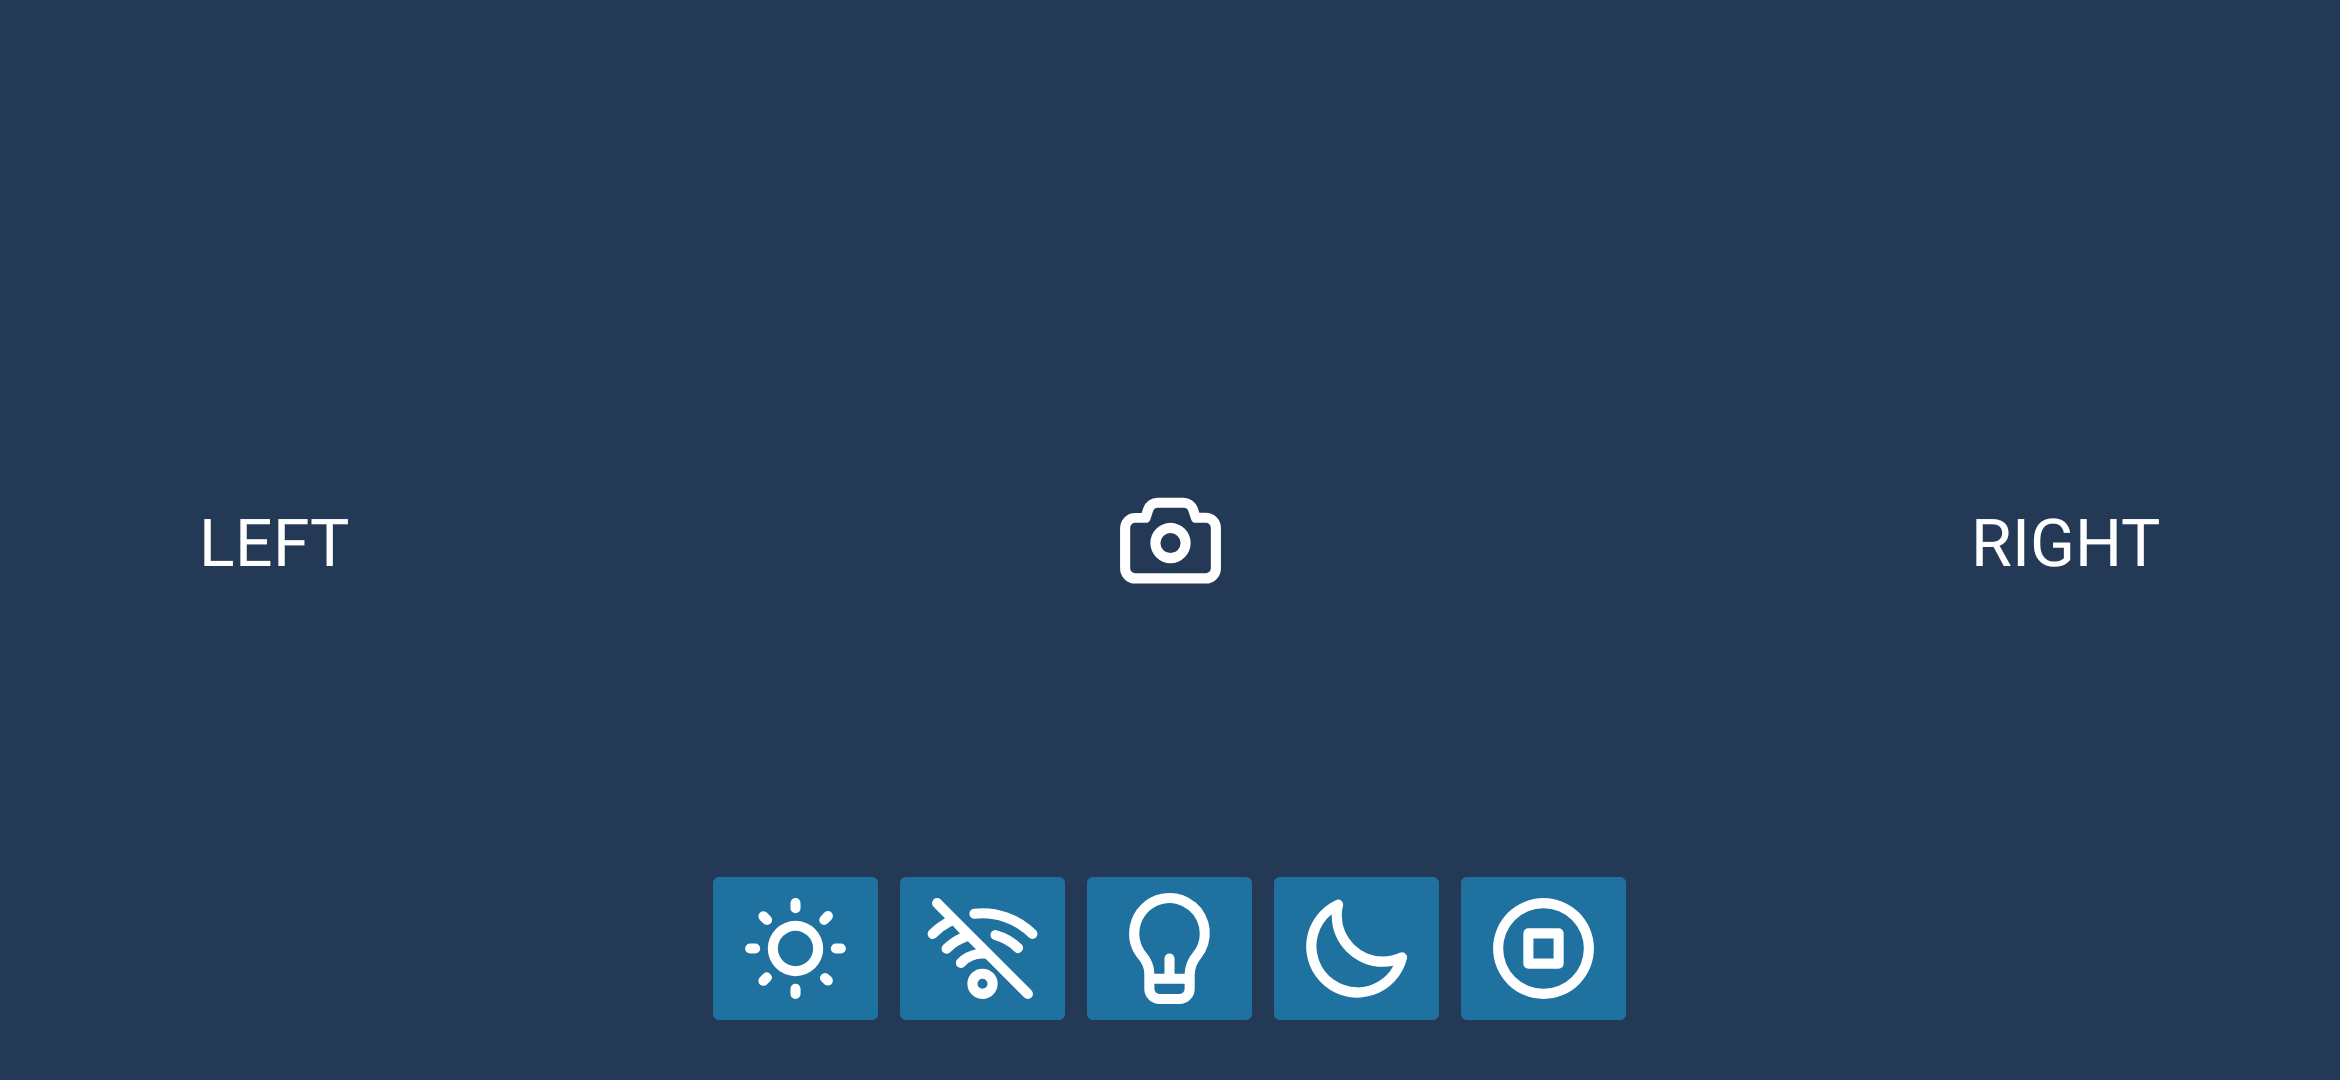
\includegraphics[scale=.1]{imaxes/layout-horizontal1.png}
  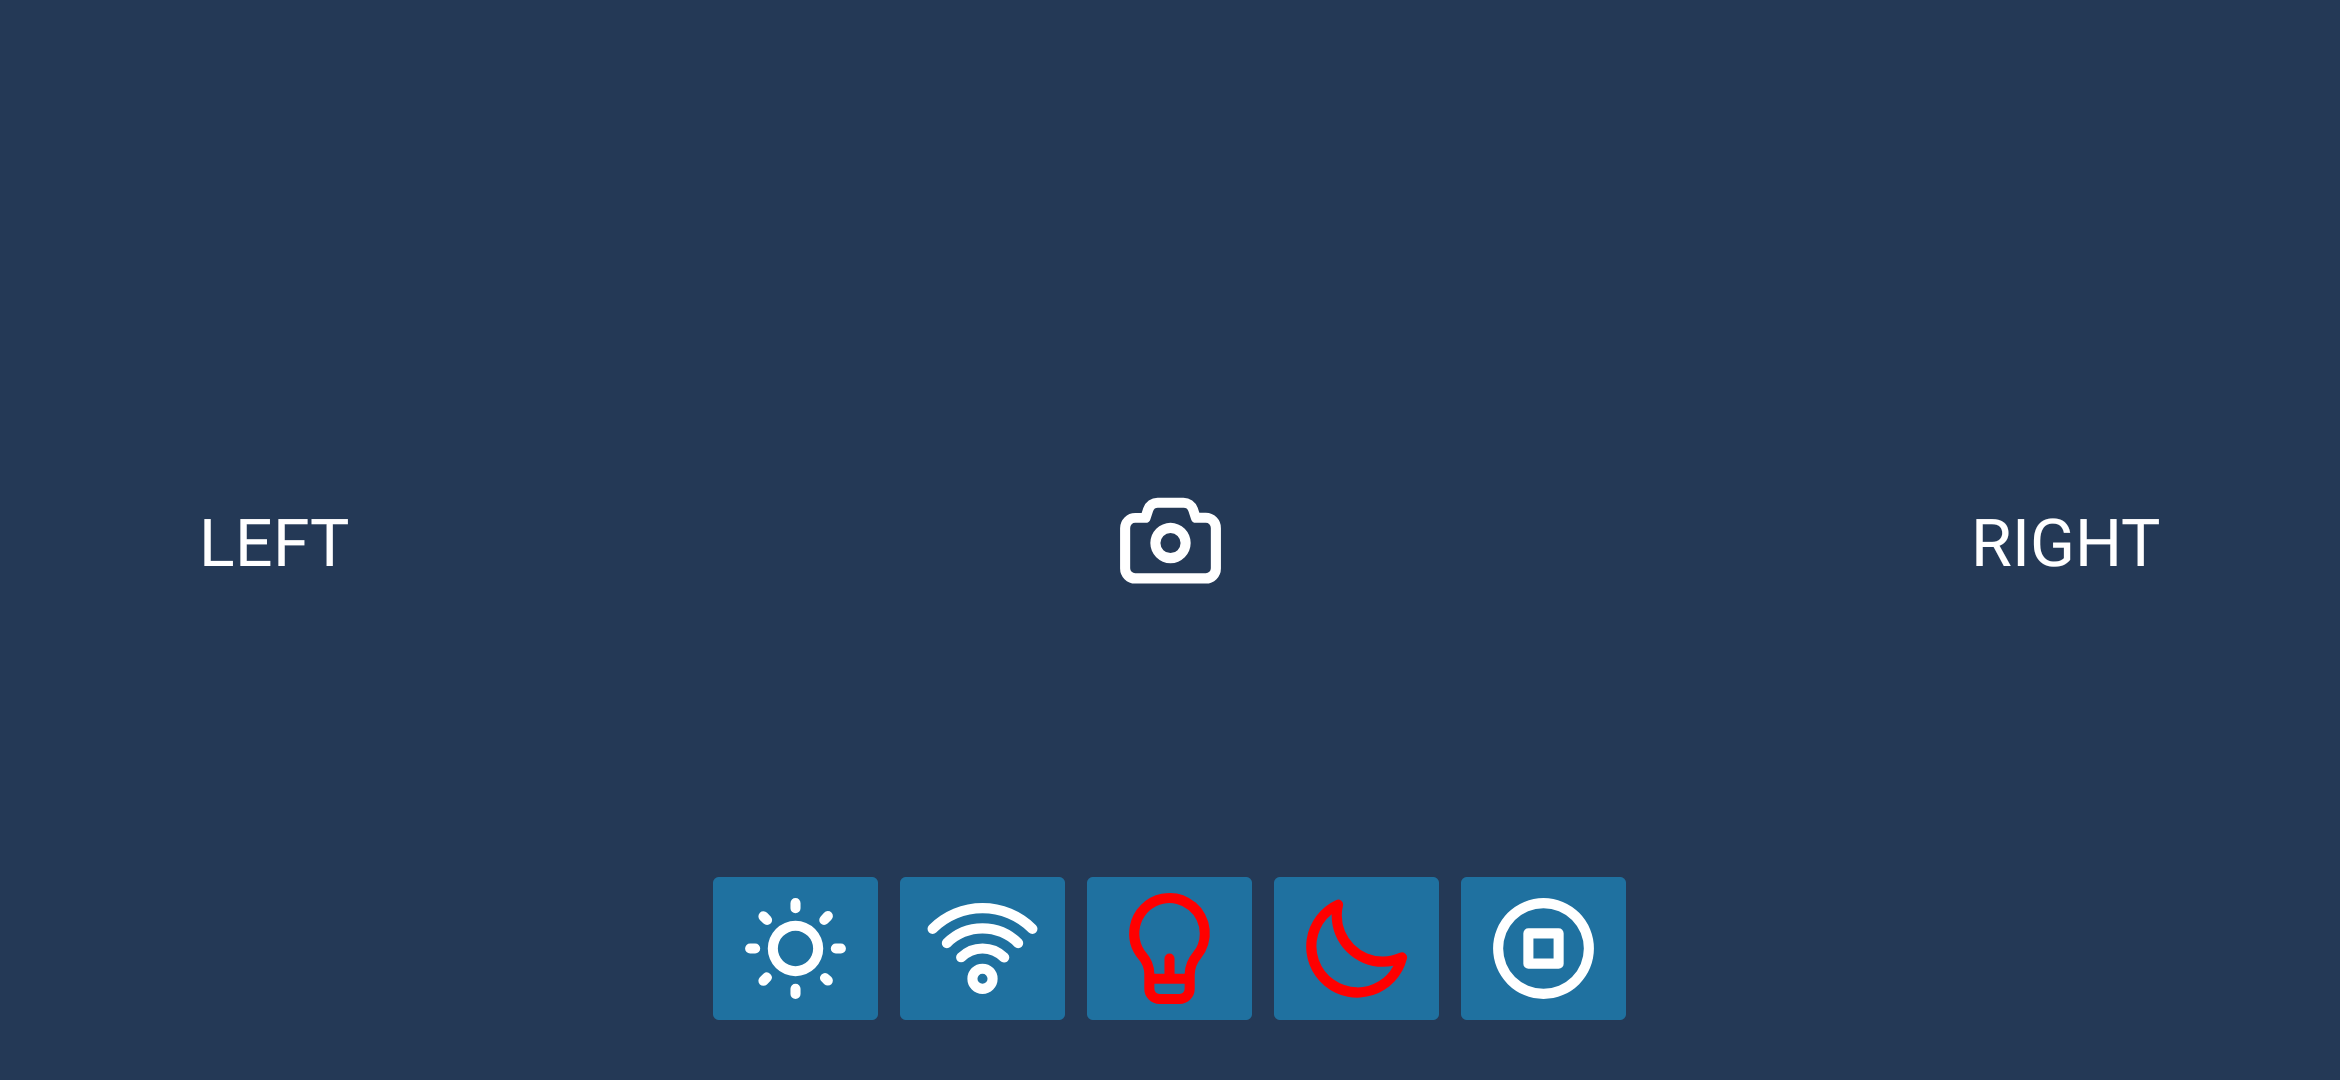
\includegraphics[scale=.1]{imaxes/layout-horizontal2.png}
  \caption{Capturas de pantalla do \emph{layout} vertical.}
  \label{f:layout vertical}
\end{figure}
\subsection{Ciclo de vida da actividade}
En Android cada actividade conta conta cun ciclo de vida, pasa por varios estados dende antes de iniciarse ata despois de finalizar. O estado principal dunha actividade é activa, no momento que a actividade está en primeiro plano e interactuando co usuario.

\begin{figure}[tb]
  \centering
  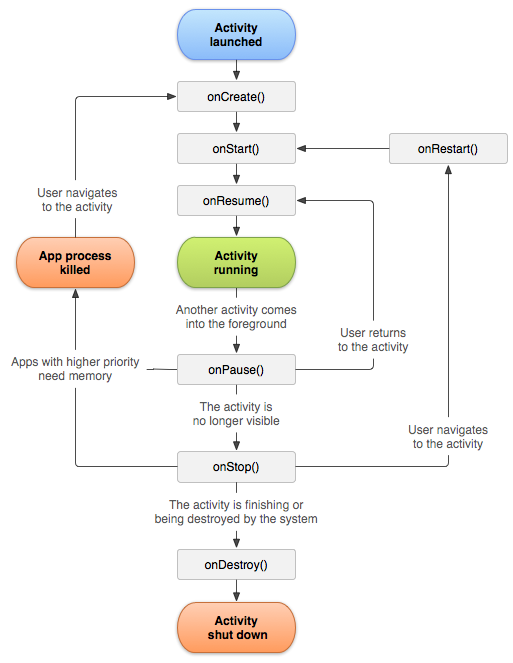
\includegraphics[scale=.6]{imaxes/ciclo-actividade.png}
  \caption{Ciclo de actividade Android (incluir referencia)}
  \label{f:actividade}
\end{figure}

Para xestionar o que sucede no resto de estados utilízanse unhas funcións de \emph{callbacks}, no noso caso realizarase as seguintes accións en cada fase:
\subsubsection{onCreate}
Este método e o que se chama ao executar a actividade. Nel iniciarase os compoñentes a mostrar en pantalla e definirase o seu comportamento.

Aquí xestionarase o estado da conexión, iniciando a clase \emph{request} se non esta en funcionamento e enviando mensaxes o dispositivo para comprobar que segue conectado. Tamén xestionarase o estado da transmisión de vídeo xa que será necesario iniciar a recepción antes de iniciar a transmisión.
\subsubsection{onResume}
Este método executase despois de \emph{onCreate} cando a pantalla xa é visible para o usuario.

Rexistrarase aquí un \emph{sensor listener} para obter a información do sensor de luz.
\subsubsection{onPause}
Este método executase cando a aplicación deixa de estar en primeiro plano, se o usuario a minimiza u outra aplicación executase a actividade pasará a \emph{onStop} se despois de acceder a aplicacións recentes a aplicación volve a primeiro plano pásese o método \emph{onResume}.

Levarase a cabo neste método a cancelación do rexistro do sensor xa que non se seguira a utilizar e deterase a transmisión de vídeo se estase a executar.
\subsubsection{onDestroy}
Neste método a actividade e detida completamente e devénse liberar os recursos.

Aquí enviarase a orde para deter a conexión co dispositivo.

\subsection{Botones}
A actividade é a encargada de iniciar os botóns e manexar o seu funcionamento. Estes botón son os seguintes:
\begin{itemize}
    \item \textbf{Esquerda:} O pulsar este botón enviarase unha orde de acender a luz de xiro a esquerda. Se hai algunha luz acesa se enviará primeiro unha orde para apagalas. O pulsalo por segunda vez se enviara a orde de apagar luz de xiro e no caso de que a luz vermella estivese acesa antes de indicar o xiro esta luz se acenderá de novo. O botón palpebrará en amarelo mentres estea aceso.
    \item \textbf{Dereita:} O seu funcionamento é o mesmo que no botón esquerda.
    \item \textbf{Vermello:} O pulsalo enviarase unha orde para acender a luz de vermella, o pulsador non funcionara se algunha das luces de xiro está acesa.
    \item \textbf{Noite:} O pulsalo activarase o modo noite, no que o sensor lumínico do móbil encargarase de acender a luz vermella cando a luz ambiente baixe de certo umbral.
    \item \textbf{Freo:} Activa o modo de freada no que acenderase a luz vermella progresivamente cando o acelerómetro do dispositivo móbil detecte unha redución súbita na velocidade.
    \item \textbf{Brillo:} Este botón despregará unha barra cun indicador que poderase deslizar para elixir a intensidade das luces.
    \item \textbf{Conexión:} Este botón enviará unha orde de conexión, unha vez conectado cambiará a súa aparencia para indicar que existe conexión co dispositivo.
\end{itemize}
\subsection{Sensores}
Unhas das vantaxes de utilizar un dispositivo móbil é que estes contan con diversos sensores para moitos fins. No noso caso utilizarase o acelerómetro e o xiroscopio para rexistrar cambios na posición e aceleracións no dispositivo e o sensor de luz para medir a intensidade de luz no ambiente.
En Android accedese o sensor instanciando a clase \emph{SensorManager} e definindo unha instancia do sensor da que obterase os datos mediante a función \emph{on sensor change}.

\subsubsection{Sensor de Luz}
O sensor de luz é un fotorreceptor que xera unha sinal eléctrica dependendo da incidencia de fotóns. Para utilizar o sensor rexistrarase un \emph{sensor listener} no método \emph{onResume} e o método de \emph{callback} \emph{onSensorChanged} executarase cada vez que se detecte un cambio, neste método definirase o comportamento do sensor: Cando o botón de Noite esta activado acenderase o botón Vermello se o sensor rexistra un valor inferior a 400 lúmines. Este valor correspondese coa intensidade lumínica o comenzo do solpor.
incluir referencia
\subsubsection{Acelerómetro e xiroscopio}
Para poder indicar a freada da bicicleta utilizarase o acelerómetro do dispositivo co que medirase a deceleración. O acelerómetro proporciona o valor da aceleración en $m/s^2$, para simplificar os cálculos utilizarase o sensor virtual \emph{ linear accelerometer} que proporciona o valor da aceleración excluíndo a gravidade asi o valor será 0 nos tres eixos cando o dispositivo este en repouso ou movéndose a unha velocidade constante.

A forza a obter é a deceleración no sentido da marcha, para poder calculala é necesario coñecer a orientación do dispositivo co respecto ao eixo lonxitudinal da bicicleta. Como se mostra na figura 4.3 o dispositivo situarase no guiador da bicicleta en dúas posición horizontal, ou vertical polo que en ámbalas dúas poderase excluír os valores dun dos eixos do acelerómetro, \emph{x} e \emph{y} respectivamente. Para coñecer a influenza dos outros dous eixos sobre o plano paralelo a bicicleta necesitamos coñecer o ángulo que forma con esta. Utilizaremos o sensor virtual \emph{game rotation vector} para obter este ángulo, este sensor utiliza os datos do acelerómetro e o xiroscopio para proporcionar valores rotación en radiáns sobre os eixo de coordenadas da terra, aínda que non orientado o norte xa que este sensor virtual non utiliza o magnetómetro.  Estes valores están expresados en ángulos de Euler que indican mediante unha sucesións de xiros a desviación do sistema de coordenadas, para obter o ángulo respecto o eixo de coordenadas do móbil transformaremos o vector obtido mediante o calculo a matriz de rotación. Unha vez obtidos valores normalizados utilizaremos o ángulo respecto o eixo \emph{x} se o móbil esta en posición vertical e con respecto a \emph{y} se está en horizontal.

O ángulo obtido coincide co ángulo con respecto o eixo direccional da bicicleta so no caso no que a bicicleta estea sobre chan plano polo que será necesario que a bicicleta estea sobre un terreo sen inclinación, para elo o cálculo do ángulo realizarase nun proceso de calibración, cando se acenda o modo freada solicitarase que se coloque o telefono no soporte do guiador e se suxeite a bicicleta sobre un terreo chairo.
\begin{figure}[tb]
  \centering
  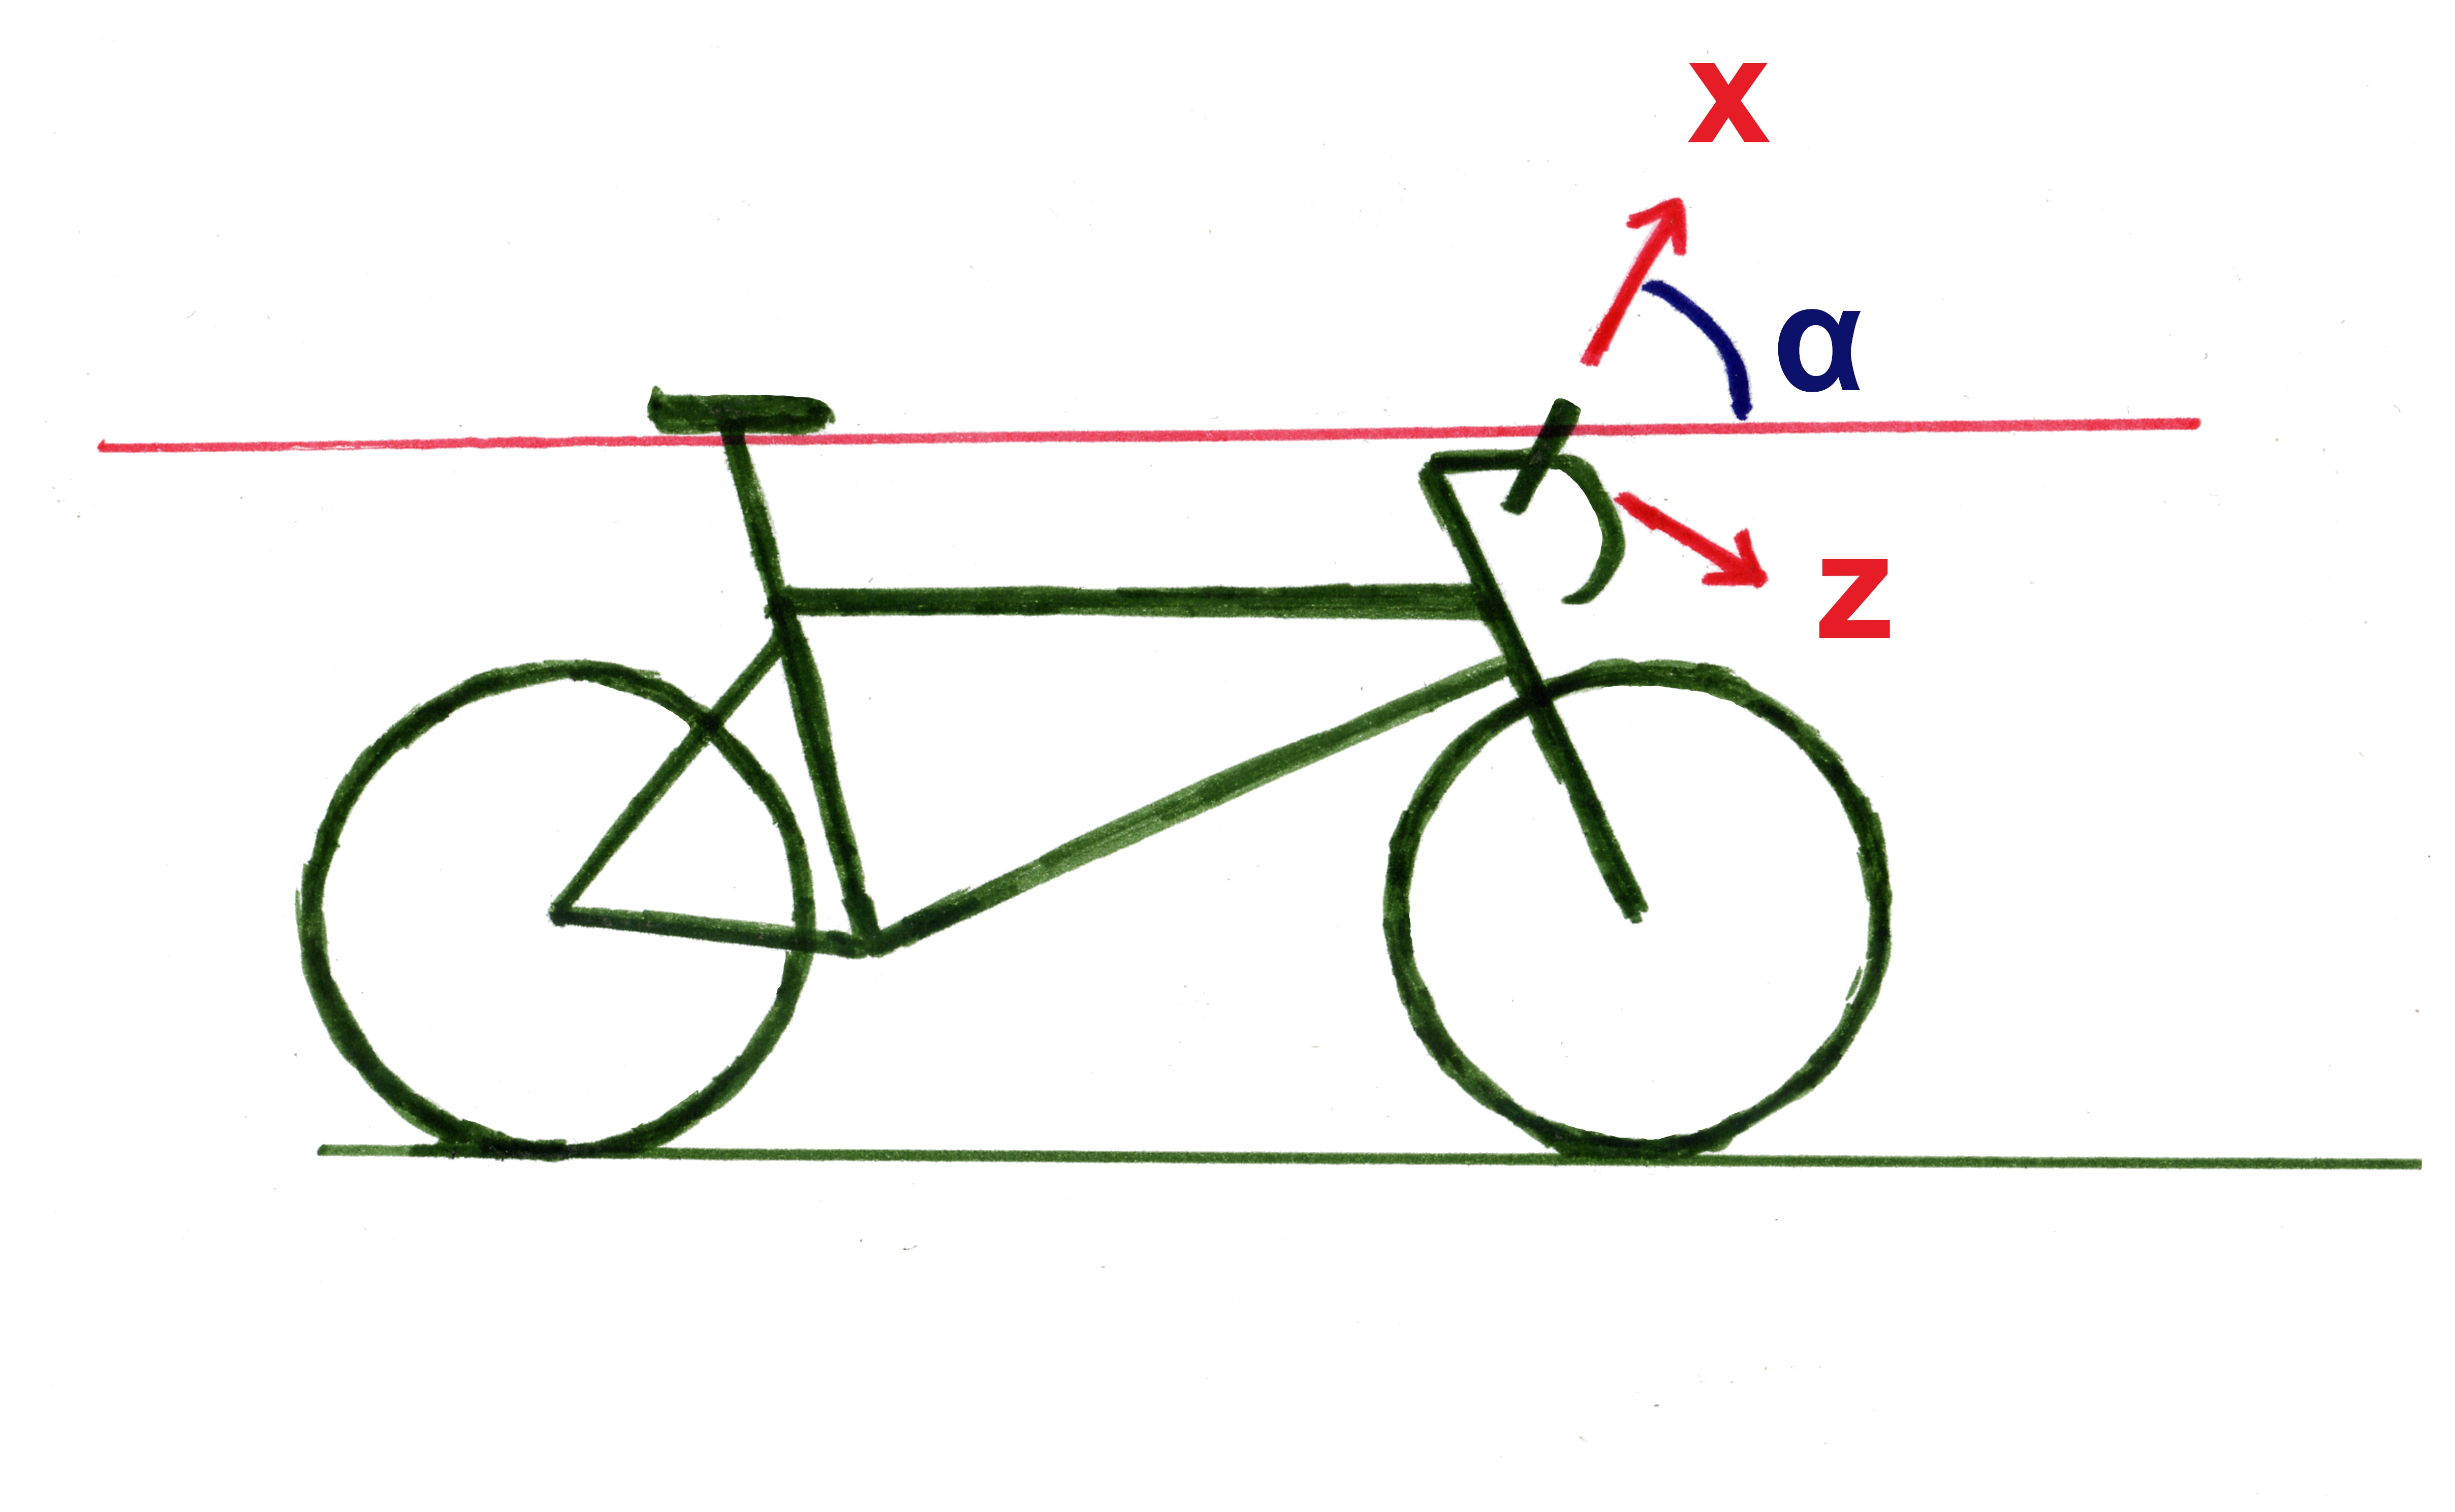
\includegraphics[scale=.6]{imaxes/angulo.png}
  \caption{Eixos do acelerómetro e ángulo coa horizontal. Para o dispositivo colocado en horizontal, en vertical o eixo superior sería \emph{y}.}
  \label{f:angulo}
\end{figure}

O modulo da forza resultante calcularase de forma trigonométrica a partir dos valores de aceleración dos dous eixos e o ángulo obtido. O sistema indicará que se acenda as luces cando o valor calculado supere certo nivel, utilizarase en principio o valor de $m/s^2$ e comprobarase nas probas se é o valor adecuado.

De igual forma que no sensor de luz estes sensores rexistraranse no método \emph{onResume} e os cálculos cos valores obtidos realizaranse no método \emph{onSensorChanged}.

\subsection{Superficie de vídeo}
Iniciarase a superficie de vídeo na fase de creación da aplicación, procederase a reflectir a superficie para facer un efecto de espello para facer mais natural a a visualización do vídeo. O vídeo asignarase a superficie iniciando a clase \emph{VideoReceiver} mediante as funcións de \emph{callback} que se executarán cando se produza un cambio na superficie de vídeo.

\section{Comuniciacíon co dispositivo}
Crearase unha clase \emph{Request} encargada de tódalas comunicacións co dispositivo.  Esta clase, unha vez instanciada, encargarase de establecer a conexión co dispositivo, reconectar se se perde a conexión e transmitirlle as ordes.

\subsection{Broadcast}
Para coñecer a dirección IP do servidor, a clase \emph{request} conta cunha función que abrirá un socket no porto 5555 para esperar a recepción dun datagrama broadcasteado a tódalas direccións. O recibir o datagrama comprobase que conten a mensaxe \emph{"BikeView"} se é asi a función devolverá a dirección IP emisora do paquete.

\subsection{Conexión}
Unha vez obtida a dirección IP a clase \emph{request} utilizará unha función para establecer a conexión que devolverá un socket conectado ao socket remoto do servidor.

\subsection{Transmisión de ordes}
Para transmitir as ordes a clase \emph{request} contara cunha función que recibe a mensaxe a transmitir e a envía a través do socket. Espera a recibir resposta do servidor e se é positiva devolve o valor booleano verdadeiro, en caso de non recibila devolve o valor falso.

\section{Recepción de vídeo}
Para este apartado crearase a clase \emph{VideoReceiver} que executarase no seu propio \emph{thread}. O vídeo é codificado no formato H.264 e transmitido por UDP, para recibilo ábrese un \emph{socket} no porto 5000 extraese a mensaxe do datragrama e, para acelerar o proceso, en vez de utilizar a función \emph{MediaExtractor} pásase a unha función de parseo encargada de separar os datos recibidos en \emph{NAL units}, o formato que utiliza H.264 para o transporte. Para elo cando se identifica a cabeceira da seguinte \emph{NAL units} a anterior se envía a outra función encargada de decodificar o vídeo mediante un \emph{MediaCodec}, finalmente o vídeo mostrase na superficie.

\section{Anclaxe a bicicleta}
Existen diversas opcións paras suxeitar o móbil o guiador dunha bicicleta, no mercado hai soportes para dispositivos concretos e outros que se adaptan ao tamaño e forma de diferentes modelos. Neste caso utilizarase unha código \emph{SCAD} que ao executalo co software de deseño 3D paramétrico OpenSCAD no que introdúcense as dimensións do dispositivo e como resultado obtense un arquivo \emph{STL} co deseño 3D do soporte.
\begin{figure}[tb]
  \centering
  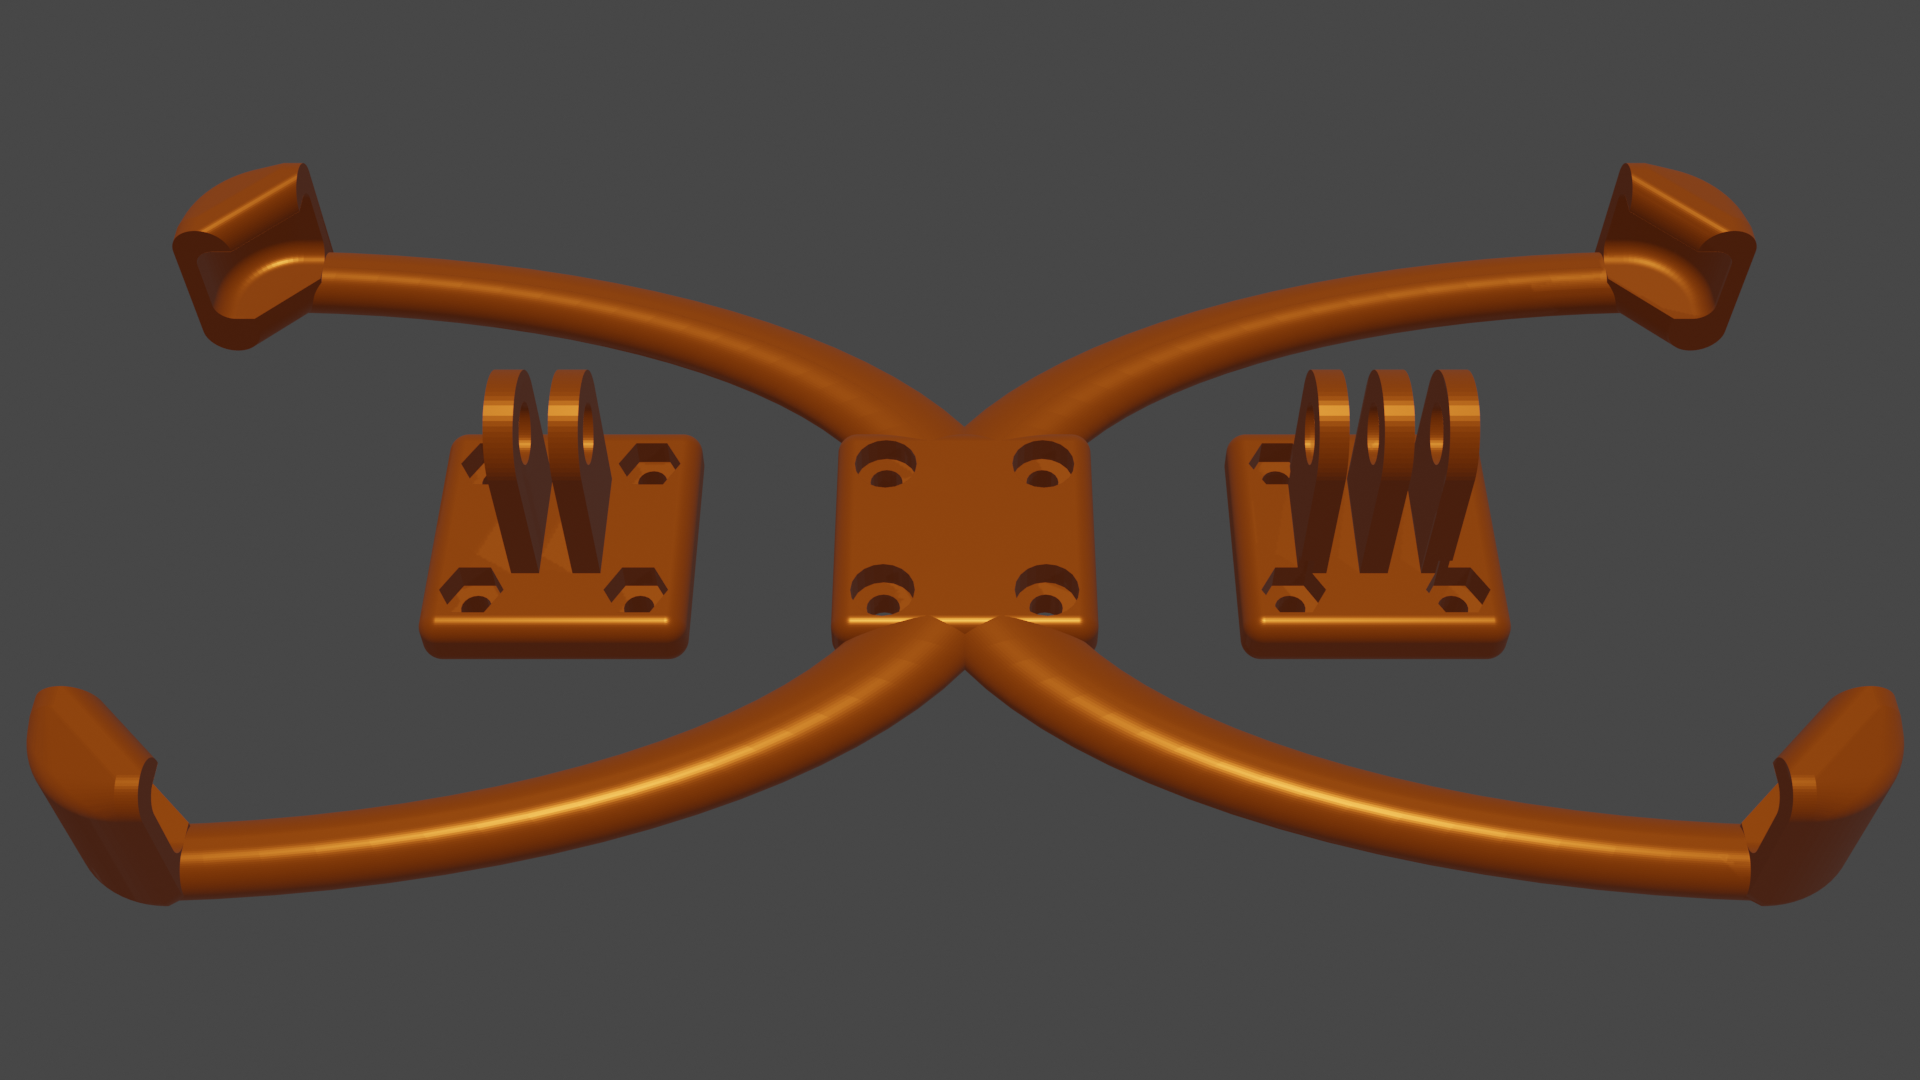
\includegraphics[scale=.2]{imaxes/soporte-mobil.png}
  \caption{Desño 3D do soporte para o dispositivo móbil.}
  \label{f:soporte móbil}
\end{figure}
Vendo que os soportes impresos non constaban coa resistencia esperada, como se mostra nas imaxes da figura  ,optouse por utilizar un soporte de aluminio nas probas para preservar a integridade do dispositivo móbil.
\begin{figure}[tb]
  \centering
  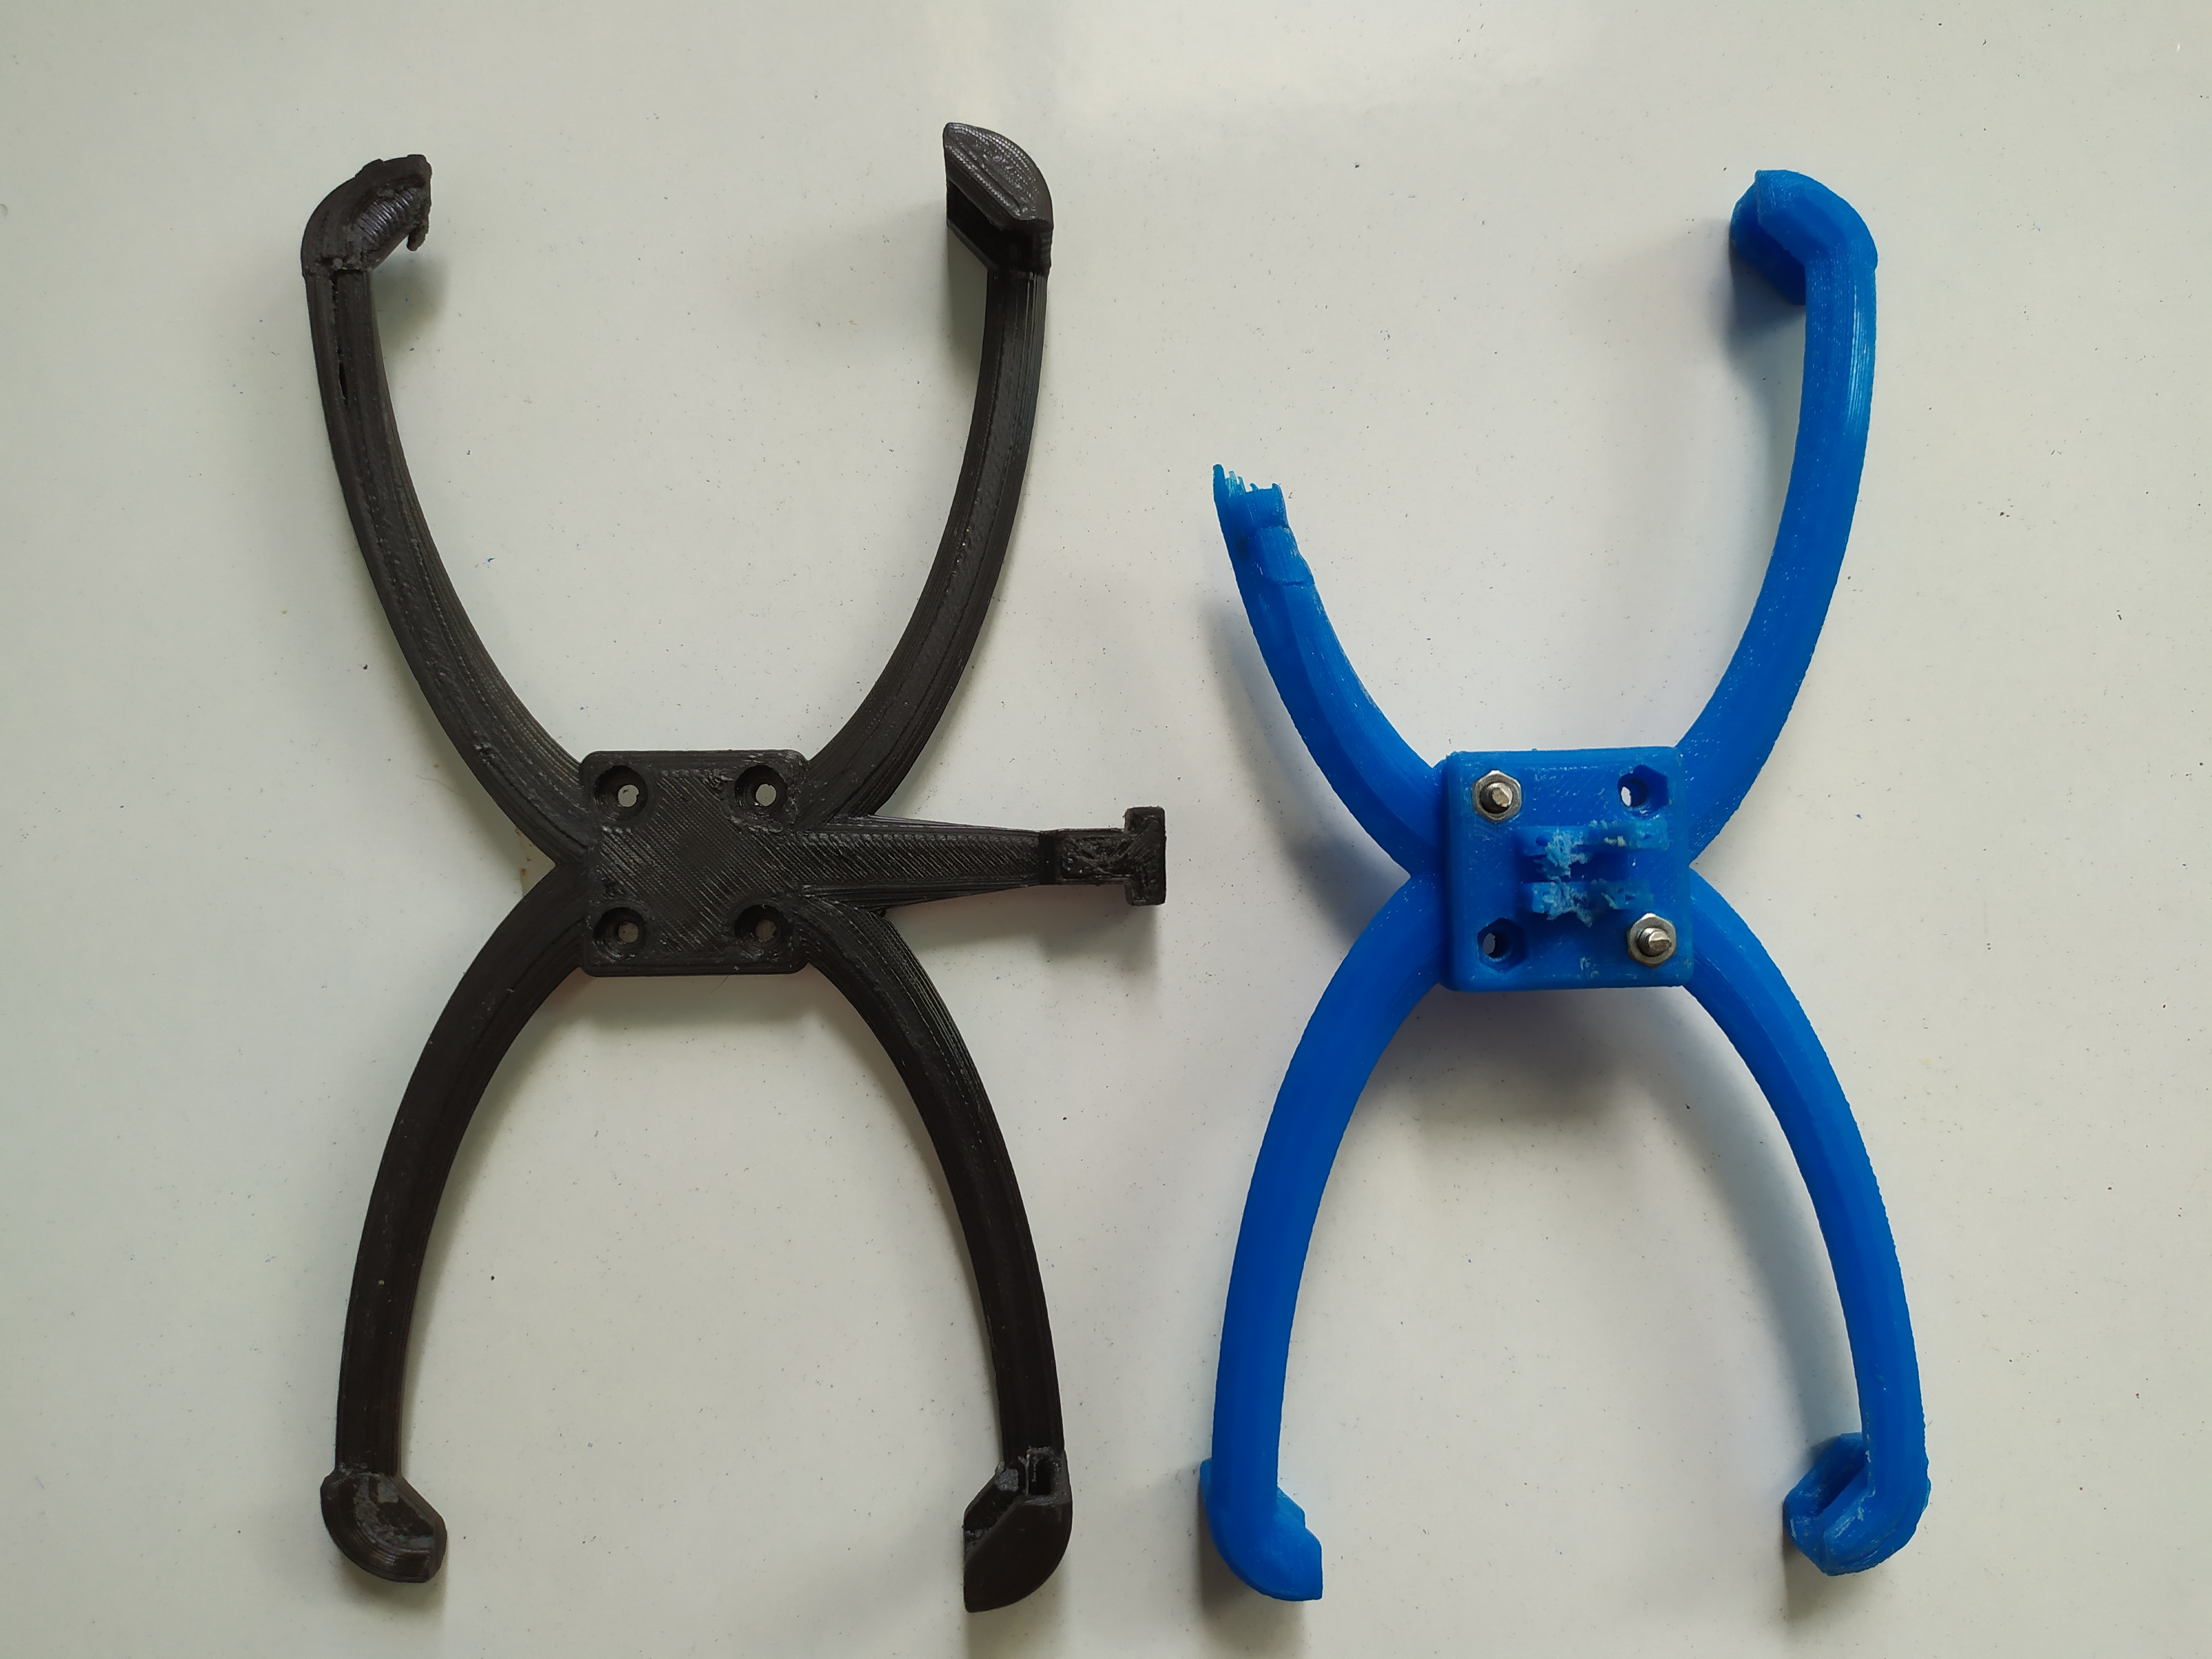
\includegraphics[scale=.08]{imaxes/fallos-soporte.jpg}
  \caption{Mostras dos problemas do soporte impreso.}
  \label{f:soporte móbil}
\end{figure}
